\documentclass[10pt]{beamer}
%\documentclass[10pt, aspectratio=169]{beamer}

\usetheme[progressbar=frametitle]{metropolis}
\usepackage{appendixnumberbeamer}
\usepackage[ngerman]{babel}
\usepackage[utf8]{inputenc}

\usepackage{booktabs}
\usepackage[scale=2]{ccicons}

% package for url
\usepackage{hyperref}

\usepackage{pgfplots}
\usepgfplotslibrary{dateplot}

\usepackage{xspace}
\newcommand{\themename}{\textbf{\textsc{metropolis}}\xspace}

\usepackage{blindtext}
\usepackage{graphicx}
\usepackage{comment}
\usepackage{mathtools}
\usepackage{amsmath}
\usepackage{amssymb}
\usepackage{proof}
\usepackage{tabularx}
\renewcommand{\figurename}{Abb.}
\usepackage{marvosym}

\definecolor{ExColor}{HTML}{17819b}
%\DeclareMathOperator{\mod}{mod}
\newcommand{\emptyWord}{\varepsilon}
\newcommand{\SigmaStern}{\Sigma^{*}}
\newcommand{\absval}[1]{|#1|}

\setbeamertemplate{footline}[text line] 
{\parbox{\linewidth}{Fachgruppe Informatik\hfill\insertpagenumber\hfill Vorkurs Theoretische Informatik\vspace{0.2in}}}



%\usepackage[OT1]{eulervm}

\title{Vorkurs Theoretische Informatik}
\subtitle{Einführung in die Grundideen und in die Mengenlehre}
\date{Montag, 30.09.2019}
\author{Arbeitskreis Theoretische Informatik}
\institute{Fachgruppe Informatik}
% \titlegraphic{\hfill\includegraphics[height=1.5cm]{logo.pdf}}

\begin{document}

\maketitle

\begin{frame}[fragile]{Übersicht}
  \setbeamertemplate{section in toc}[sections numbered]
  \tableofcontents%[hideallsubsections]
\end{frame}

\section{Allgemeines} 

\subsection{Organisatorisches}
\begin{frame}[fragile]{Wer sind wir?}
    \begin{itemize}
        \item 
            Fachgruppe Informatik
            \begin{itemize}
                \item Unser Ziel: \\
                Das Leben der Studierenden während ihres Studiums angenehmer zu gestalten
                \item vertreten die studentische Sicht in offiziellen Gremien
                \item verleihen Prüfungen aus den früheren Semestern
                \item organisieren Veranstaltungen (Spieleabende, Vorkurse, ...)
            \end{itemize}
        \item AK Theo
        \begin{itemize}
            \item Teilmenge der Fachgruppe Informatik
            \item haben diesen Vorkurs organisiert
        \end{itemize}
    \end{itemize}
\end{frame}

\subsection{Tipps zum Studium}
\begin{frame}[fragile]{Tipps zum Studium}
    \begin{itemize}
        \item Nützliche Links:\\
            \begin{itemize}
                \item Fachgruppe Informatik:\\
                \url{https://fius.informatik.uni-stuttgart.de/}
                \item Foliensätze:\\ \url{https://fius.informatik.uni-stuttgart.de/dienste/theo-vorkurs/}
                 \item Ergänzung Theoretische Informatik 1 (Wintersemester 18/19): \\
                 \url{www.fmi.uni-stuttgart.de/ti/teaching/w18/eti1/}
            \end{itemize}
        \item E-Mail der Fachgruppe: fius@informatik.uni-stuttgart.de
            
    \end{itemize}
\end{frame}


\section{Theoretische Informatik}

\subsection{Anwendung}
\begin{frame}[fragile]{Was ist eigentlich Theoretische Informatik?}
    \begin{itemize} 
    \item Theoretische Informatik ist die \textbf{formale} Herangehensweise an Probleme.\\
    \item Diese Probleme befassen sich unter Anderem mit den \textbf{formalen} Sprachen.
    \end{itemize}
\end{frame}

\begin{frame}{Anwendung der theoretischen Informatik}
    \begin{itemize}
        \item Ist ein bestimmtes Problem lösbar, oder \textbf{können} wir gar keine Lösung finden?
        \item IT-Sicherheit / Kryptographie: Die Sicherheit bestimmter Algorithmen \textbf{beweisen}
        \item Reguläre Ausdrücke
        \item Künstliche Intelligenz
        \item Compilerbau
        \item ...und vieles mehr...
    \end{itemize}
\end{frame}

\subsection{Theoretische Informatik in deinem Studium}
\begin{frame}[fragile]{Theoretische Informatik in deinem Studium}
Theoretische Informatik I ist Orientierungsprüfung für Informatik, Medieninformatik, Softwaretechnik und Data Science.
    \begin{itemize} 
    \item Du musst diese Prüfung spätestens zum Ende des dritten Semester bestanden haben.
    \item Du musst spätestens zum Ende des zweiten Semesters eine der beiden Orientierungsprüfungen angetreten haben.
    \item Du kannst die schriftliche Prüfung einmal nachschreiben und hast dann noch einen mündlichen Versuch im selben Semester.
    \end{itemize}
    \alert{Kennt eure Prüfungsordnung!}
\end{frame}

\begin{frame}{Theoretische Informatik in deinem Studium}
    \begin{itemize}
        \item Theoretische Informatik I\\
        Formale Sprachen und Automatentheorie (FSuA)
        \item Theoretische Informatik II\\
        Berechenbarkeit und Komplexität (BuK)
        \item Theoretische Informatik III\\
        Algorithmen und Diskrete Strukturen (AuDS)
    \end{itemize}
\end{frame}

\begin{frame}{Literatur der Vorlesung}
    \small{Uwe Schöning: Theoretische Informatik - kurzgefasst [\only<1>{22,99}\only<2>{\alert{0}}€]\\
    \begin{itemize}
        \item Die Vorlesung von Prof. Hertrampf richtet sich in weiten Teilen nach diesem Buch.
    \end{itemize}
    Boris Hollas: Grundkurs Theoretische Informatik: Mit Aufgaben und Anwendungen [\only<1>{27,99}\only<2>{\alert{0}}€]\\
    \begin{itemize}
        \item Weniger formal, dafür intuitiver mit einigen Beispielen und Übungsaufgaben
    \end{itemize}
    Dirk W. Hoffmann: Theoretische Informatik
    \begin{itemize}
        \item wird von Joel oft empfohlen
    \end{itemize}}
    
\onslide<2>{\alert{Die Bücher sind alle in der Uni-Bib verfügbar, beim Schöning sollte man sich aber beeilen.}}
\end{frame}

\section{Wörter, Sprachen und Mengen}

\begin{frame}[fragile]{Mengen}
    \begin{itemize}
        
        \item<1->
            Was ist eine \alert<1,2>{Menge}?
        \item<2->
            \only<2>{
            \vspace*{0.5cm}
                Eine Menge
                \begin{itemize}
                    \item ist eine \alert{Sammlung von Zeugs}
                    \item ist unsortiert
                    \item enthält keine Duplikate
                    \item wird mit geschweiften Klammern notiert
                \end{itemize}
                
                \metroset{block=fill}
                
                \begin{exampleblock}{Beispiel}
                    $\mathbb{N} = \{0, 1, 2, 3, \dots \}$ = Menge der Natürlichen Zahlen\\
                    Studenten = \{Janette, Julian, Joel, Fabian, $\dots$\}\\
                    $\{1,2\} = \{2,1\} = \{1,1,2,1,1,1\}$\\
                    $\emptyset = \{\} =$ leere Menge
                \end{exampleblock}}
            \uncover<3->{
            Was ist ein \alert<3,4>{Element}?}
        \item<4->
        \only<4>{
            \vspace*{0.5cm}
            Ein Element ist ein \alert{Ding aus einer Menge}.\\
            
            \metroset{block=fill}
                
            \begin{exampleblock}{Beispiel}
                $\mathbf{1}$ ist ein Element der \textbf{Natürlichen Zahlen}\\
                $\mathbf{1} \in \mathbb{N}$\\
                \vspace*{0.5cm}
                \textbf{Janette} ist ein Element aus der Menge der \textbf{Studenten}\\
                \textbf{Janette} $\in$ \textbf{Studenten}\\
                \vspace*{0.5cm}
                $\mathbf{a}$ ist in der Menge $\mathbf{\{u, v, w\}}$ nicht enthalten\\
                $\mathbf{a} \notin \mathbf{\{u, v, w\}}$
            \end{exampleblock}
        }
        \uncover<5->{
            Was ist eine \alert<5,6>{Teilmenge}?
        }
        \item<6>
            \vspace*{0.5cm}
            Eine Teilmenge ist eine \alert{spezielle Auswahl} von Elementen einer Menge.\\
            
            \metroset{block=fill}
            
            \begin{exampleblock}{Beispiel}
                $\{1, 2, 3\}$ ist eine Teilmenge der Natürlichen Zahlen\\
                $\{1,2,3\} \subseteq \mathbb{N}$\\
                \vspace*{0.5cm}
                \{\textbf{Janette}\} ist eine Teilmenge der \textbf{Studenten}\\
                \{\textbf{Janette}\} $\subseteq$ \textbf{Studenten}
            \end{exampleblock}
            
    \end{itemize}
\end{frame}

\begin{frame}{Mengen - Mal anders}
    \begin{alertblock}{Ein paar Definitionen}
    Eine nichtleere Menge einstelliger Symbole nennen wir \alert{Alphabet}.
    Es wird oft dargestellt durch den Bezeichner $\Sigma$.\\
    \end{alertblock}
    \metroset{block=fill}
    \begin{exampleblock}{Beispiele}
    \begin{itemize}
        \item $\Sigma = \{a,b\}$
        \item $\Sigma = \{0,1\}$
        \item $\Sigma = \{\text{Rechts, Links, Vorwärts, Rückwärts, Start, Stopp, Pause}\}$
    \end{itemize}
    \end{exampleblock}
\end{frame}

\begin{frame}[fragile]{Mengen - Mal anders}
    \begin{alertblock}{Ein paar Definitionen}
    Auf einem Alphabet können wir die Operation $\cdot$\;, genannt \alert{Konkatenation}, ausüben.\\
    $\rightarrow$ zum Beispiel ist dann $a \cdot b = ab$\\
    Eine beliebig lange Kette an Symbolen aus dem Alphabet nennen wir ein \alert{Wort}.
    \end{alertblock}
    \metroset{block=fill}
    \begin{exampleblock}{Beispiele}
    \begin{itemize}
        \item $abba$ ist ein \emph{Wort} über dem \emph{Alphabet} $\Sigma = \{a,b\}$
        \item $10011101$ ist ein \emph{Wort} über dem \emph{Alphabet} $\Sigma = \{0,1\}$
        \item StartVorwärtsRechtsVorwärtsStopp ist ein Wort über $\Sigma = \{\text{Rechts, Links, Vorwärts, Rückwärts, Start, Stopp, Pause}\}$
    \end{itemize}
    
    \end{exampleblock}
\end{frame}

\begin{frame}{Wortlängen}
    \begin{alertblock}{Wortlänge und das leere Wort}
        Eine endlich lange Kette an Symbolen aus dem Alphabet nennen wir ein Wort.
    \end{alertblock}
    \begin{itemize}
        \item Wort der Länge 3: z.B. $aaa, abc, \dots$
        \item Wort der Länge 2: z.B. $aa, ab, \dots$
        \item Wort der Länge 1: z.B. $a, b, c, \dots$
        \item Wort der Länge \alert<2>{0}: \alert<2>{$\emptyWord$}
    \end{itemize}
    \only<1>{Wir schreiben \alert<1>{$\absval{w}$} um \alert<1>{Länge des Wortes $w$} abzukürzen.\\}
    \only<2>{$\emptyWord$ \emph{(\textquotedbl Epsilon\textquotedbl)} nennen wir das "leere Wort".
    \begin{itemize}
        \item \alert{Vergleich:} Es ist vergleichbar mit einem leerem String,\\ \qquad\qquad \,\, also: $\dq\dq=\emptyWord$
        \item \alert{Achtung:} Das leere Wort kann kein Teil eines Alphabets sein,\\\qquad\qquad da es nicht einstellig ist.
    \end{itemize}}
\end{frame}

\begin{frame}{neutrales Element der Konkatenation}
    \begin{alertblock}{Achtung}
        Wir können bei der Konkatenation auch das leere Wort anhängen. Es verhält sich hierbei als das neutrale Element.\\
        d.h. für ein beliebiges Wort $a$, ist $a\cdot\emptyWord = \emptyWord\cdot a=a$
        \begin{exampleblock}{Vergleich}
        \begin{itemize}
            \item Bei der Addition von Zahlen ist die 0 das neutrale Element\\
            $a+0=0+a=a$
            \item Bei der Multiplikation von Zahlen ist die 1 das neutrale Element\\
            $a*1=1*a=a$
        \end{itemize}
        
        \end{exampleblock}
    \end{alertblock}
\end{frame}


\begin{frame}[fragile]{$\Sigma^\ast$}
%\alert{Für \Sigma = \{a,b\}}:
\begin{figure}
    \centering
    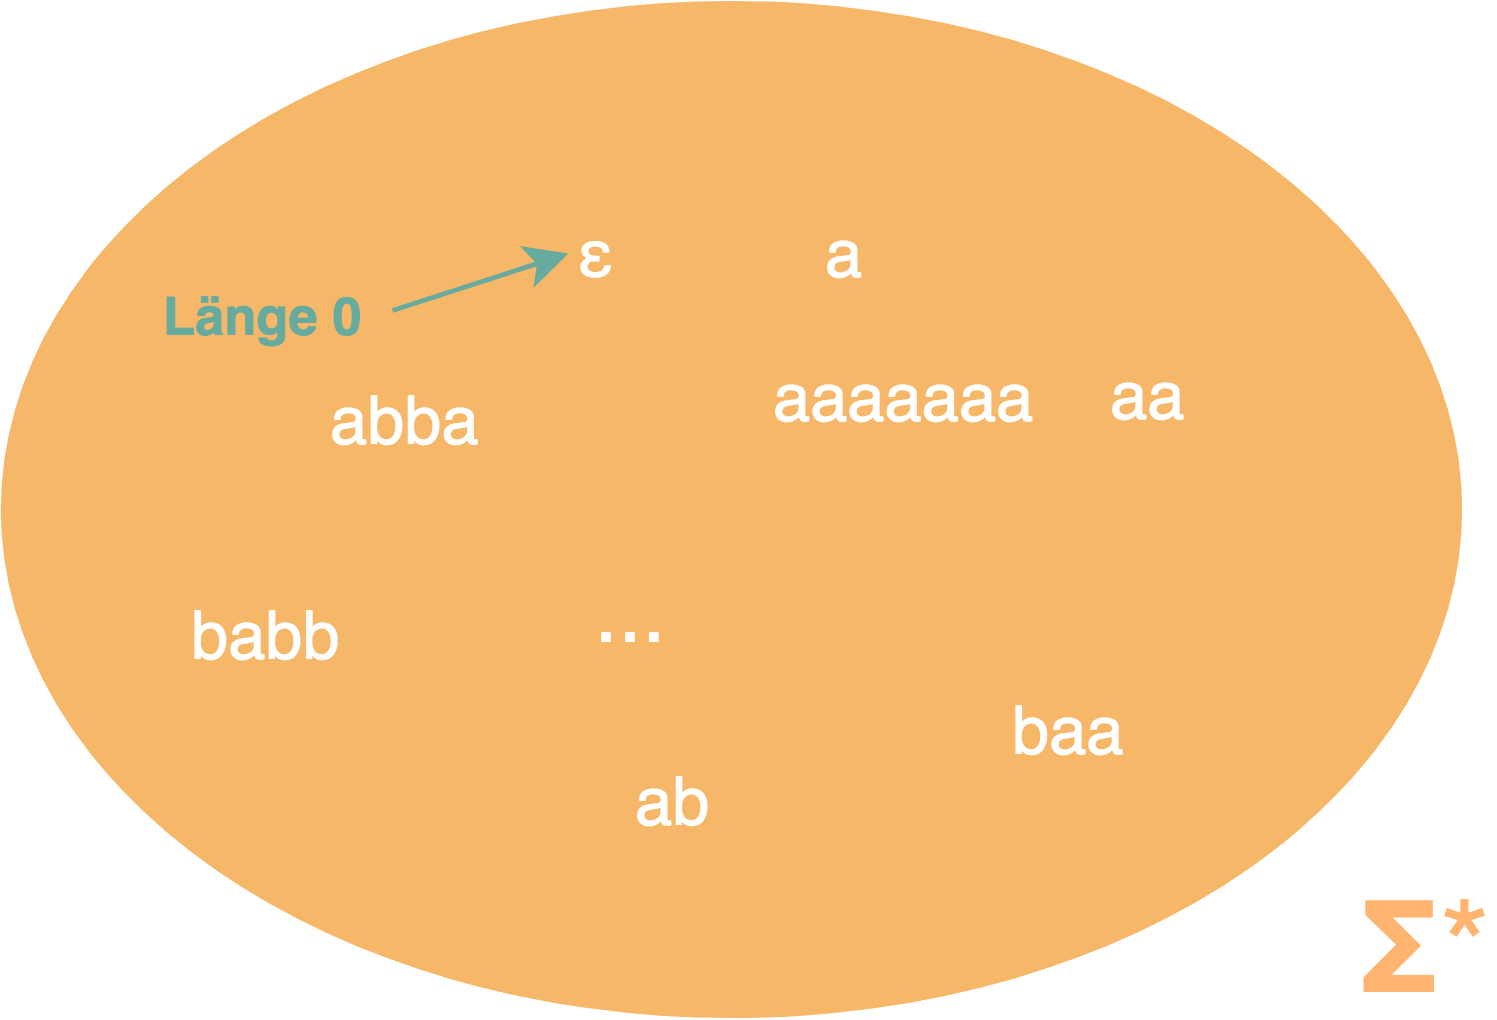
\includegraphics[width=0.7\textwidth]{figures/SigmaSternEpsilon.png}
    \caption{Menge von allen Kombinationen der Elemente von $\Sigma$ heißt $\Sigma^\ast$}
\end{figure}
\end{frame}

\begin{frame}[fragile]{$\Sigma^\ast$}
    %\metroset{block=fill}
    \begin{exampleblock}{Das heißt\dots}
    Sei $\Sigma = \{a,b\}$ unser \alert{Alphabet}.\\
    Wir beschreiben die Menge, die alle Möglichkeiten enthält Elemente aus $\Sigma$ zu \emph{konkatenieren} mit $\Sigma^\ast=\{\emptyWord,a,b,aa,ab,ba,bb,aba,\dots\}$.
    \end{exampleblock}\pause
    
    \begin{alertblock}{Achtung}
    $M^\ast$ über einer beliebigen Menge $M$ enthält immer das leere Wort $\emptyWord$!\\
    Sogar wenn $M = \{\} = \emptyset$.\\
    
    \end{alertblock}
\end{frame}

{\setbeamercolor{palette primary}{bg=ExColor}
\begin{frame}[fragile]{Denkpause}
    \begin{alertblock}{Aufgaben}
    Nenne jeweils 5 der kürzesten Elemente aus $\alert{\Sigma^{*}}$ für die folgenden Alphabete $\alert\Sigma$:
    \end{alertblock}
    
    \metroset{block=fill}
    \begin{block}{Normal}
        \begin{itemize}
            \item $\Sigma = \{a\}$
            \item $\Sigma = \{0, 1, 2, 3, 4, 5, 6, 7, 8, 9\}$
        \end{itemize}
    \end{block}
    \metroset{block=fill}
    \begin{block}{Etwas schwerer}
        \begin{itemize}
            \item $\Sigma$ = \{0, x, Bieber\}
            \item $\Sigma$ = \{\Smiley, \Frowny\}
        \end{itemize}
    \end{block}
\end{frame}
}

{\setbeamercolor{palette primary}{bg=ExColor}
\begin{frame}{Lösungen}
    Mögliche Lösungen sind \dots
  \begin{itemize}[<+- | alert@+>]
        \item $\emptyWord, a, aa, aaa, aaaa \in \{a\}^{*}$
        \item $\emptyWord, 0, 1, 2, 3\in \{0,1,2,3,4,5,6,7,8,9\}^{*}$
        \item $\emptyWord, 0, x, Bieber, xBieber \in \{0, x, Bieber\}^{*}$
        \item $\emptyWord$, \Smiley, \Frowny, \Smiley\Smiley, \Smiley\Frowny$\; \in \{$\Smiley, \Frowny$\}^{*}$
    \end{itemize}
\end{frame}
}

\begin{frame}[fragile]{Alphabete und $\Sigma^{*}$}
\begin{alertblock}{Verständnisabfrage}
    Denke kurz über folgende Aufgabe nach...
    \end{alertblock}
    
    \metroset{block=fill}
    \begin{block}{Schwer}
        Welche Wörter sind in $M^{*}$ enthalten, wenn $M = \emptyset$ gilt?
    \end{block}
\end{frame}

{\setbeamercolor{palette primary}{bg=ExColor}
\begin{frame}{Lösungen}
  \begin{itemize}
        \item In $M^{*} = \{$ $ \}^{*}$ ist \textbf{nur} das leere Wort $\emptyWord$ enthalten.
    \end{itemize}
\end{frame}
}

\begin{frame}[fragile]{Sprachen}
\begin{figure}
    \centering
    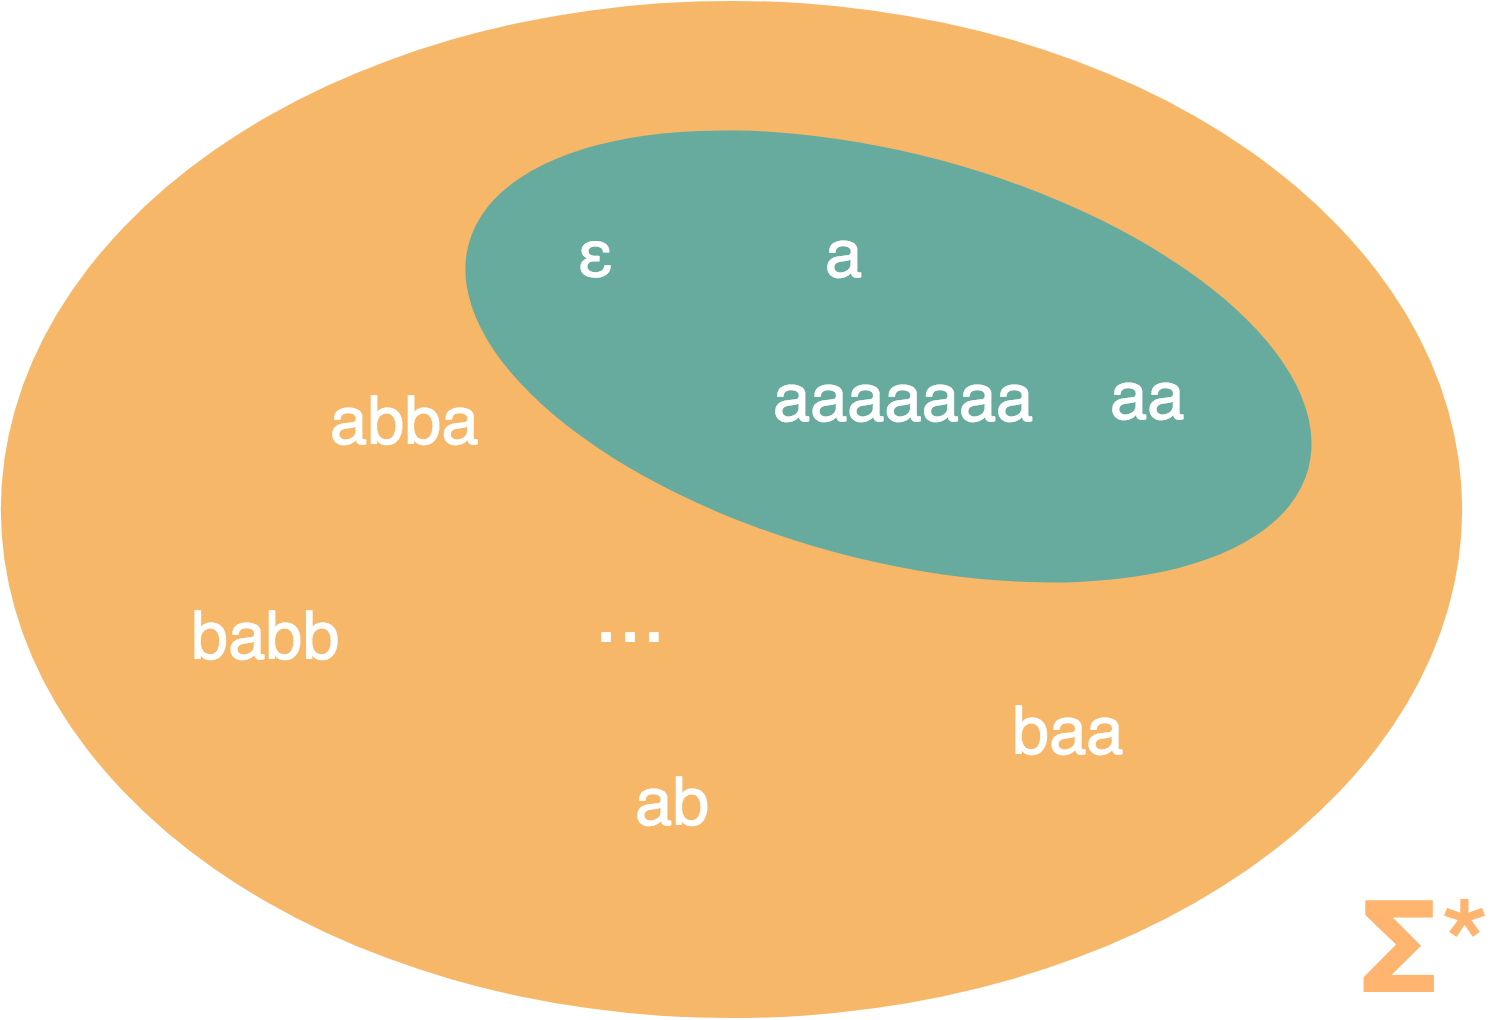
\includegraphics[width=0.7\textwidth]{figures/MysterySprache.png}
    \caption{Teilmengen unserer Obermenge nennen wir Sprachen}
    \label{fig:my_label}
\end{figure}
\end{frame}

\begin{frame}[fragile]{Sprachen beschreiben}
\begin{figure}
    \centering
    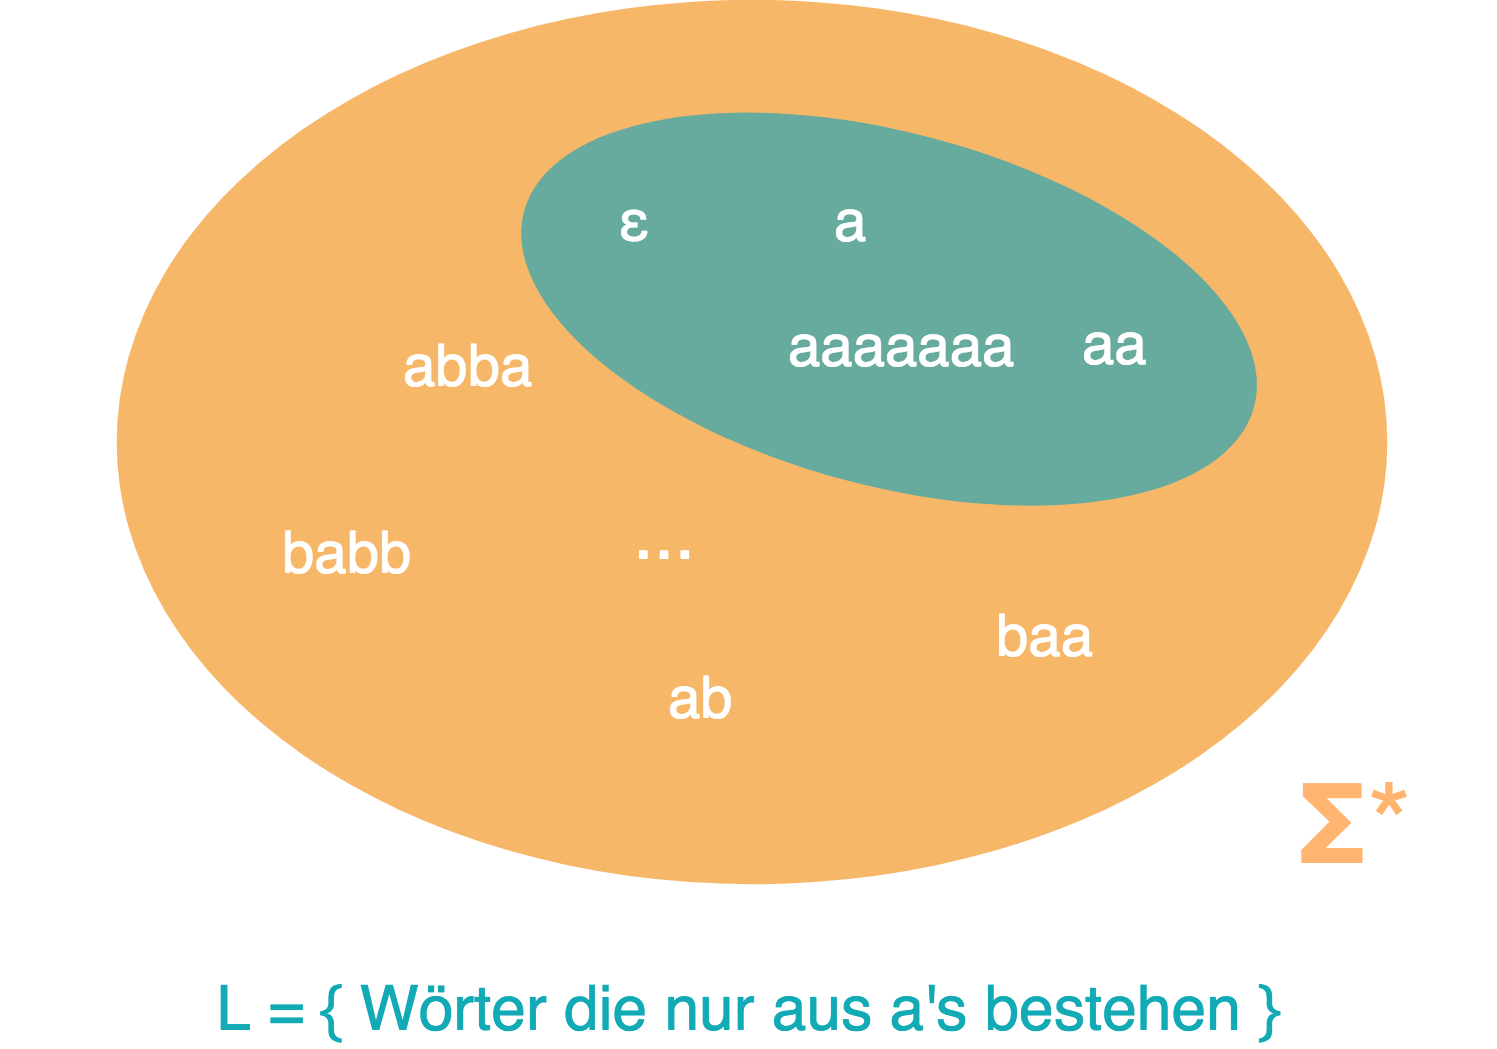
\includegraphics[width=0.7\textwidth]{figures/SprachReveal.png}
    \caption{Manche Sprachen können wir mit Regeln beschreiben}
    \label{fig:my_label}
\end{figure}
\end{frame}

\begin{frame}[fragile]{Sprachen beschreiben}
    \metroset{block=fill}
    \begin{exampleblock}{Beispiele für Sprachen in Mengenschreibweise}
    \begin{itemize}
        \item $L_1 = \{a^n\;|\;n\in\mathbb{N}\}$
        \item $L_2 = \{a^n\;|\;n \equiv 0 \bmod 2, n\in\mathbb{N}\}$
        \item $L_3 = \{uv\;|\;u\in\{a,b\}^\ast,\;v\in\{a\}\}$
        \item $L_4 = \{w\;|\;|w|_a = 3\}$
    \end{itemize}
    \end{exampleblock}
    Was soll das alles? Mehr dazu nach der Pause :)
\end{frame}

\begin{frame}[standout]
  Murmelpause
\end{frame}

\section{Mengenschreibweise} 



\begin{frame}[fragile]{Wie sprechen wir das?}
$L_2 = \{a^n \alert{\mid} n \in \mathbb{N}\}$ \\

\emph{Die Sprache $L_2$ enthält alle Wörter $a^n$, \alert{für die gilt}: n stammt aus der Menge der natürlichen Zahlen.}
\vspace{5}

\metroset{block=fill}
\begin{alertblock}{Achtung}
    In der theoretischen Informatik enthält $\mathbb{N}$ ($\mathbb{N}$ ist die Menge der natürlichen Zahlen) die Zahl 0.
\end{alertblock}

\end{frame}

\begin{frame}[fragile]{Wie schreiben wir das?}
    \begin{itemize}
        Viele Zeichen hintereinander (konkateniert) können auch einfacher geschrieben werden.
        \begin{align*}
            a^0 &= \emptyWord\\
            a^1 &= a\\
            a^2 &= a \cdot a = aa\\
            a^3 &= a \cdot a \cdot a = aaa\\
            &\vdots\\
            a^n &= \underbrace{a \cdot a \cdot ... \cdot a}_{\text{n-mal}}
        \end{align*}
        
        \end{itemize}
\end{frame}

\begin{frame}[fragile]{Wie schreiben wir das?}
    \begin{itemize}[<+- | alert@+>]
        \item $L_1 = \{0,2,4,6,8,\dots\} = \{x \mid \text{x ist gerade}\}$\\
        $L_1 = \{x \mid$ Es gibt eine Zahl $k \in \mathbb{N} : 2k = x\}$\\
        
        \item $L_2 = \{a^n \mid n \in \mathbb{N}\} = \{\emptyWord, a,aa,aaa,aaaa, \dots\}$
        
        \item $L_3 = \{a^nb^n \mid n \in \mathbb{N}\} = \{\emptyWord, ab ,aabb,aaabbb,aaaabbbb, \dots\}$
        
        \item $L_4 = \{a^nw \mid n \in \mathbb{N}, w = bccb\} = \{bccb, abccb, aabccb, \dots\}$\\
        $L_4$ endet nach einer beliebigen Anzahl von a's immer mit bccb
        
        \item $L_5 = \{w \mid |w| = 2, w\in \{a,b\}^{*}\} = \{aa,bb,ab,ba\}$\\
        Wörter der Länge 2 aus $\{a,b\}^{*}$
        
        \item $L_6 = \{w \mid |w|_a = 2, w\in \{a,b\}^{*}\}$\\
        Wörter mit \alert{genau} 2 a's aus $\{a,b\}^{*}$
    \end{itemize}
\end{frame}

{\setbeamercolor{palette primary}{bg=ExColor}
\begin{frame}[fragile]{Denkpause}
    \footnotesize
        \begin{alertblock}{Aufgaben}
            Findet Wörter aus den folgenden Sprachen
        \end{alertblock}
        \metroset{block=fill}
        \begin{block}{Normal}
            \begin{itemize}
                \item $L_1 = \{a\}$
                \item $L_2 = \{uv\;|\;u\in\{a,b\}^\ast,\;v\in\{c,d\}\}$
                \item $L_3 = \{w\;|\;|w| = 3, w\in \{a,b,c\}^{*}\}$
            \end{itemize}
        \end{block}
        \begin{block}{Etwas Schwerer}
            \begin{itemize}
                \item $L_4 = \{a^n\;|\;n \equiv 1 \bmod 3, n\in\mathbb{N}\}$
                \item $L_5 = \{w\;|\;|w|_a = 3, |w|_b = 1, w\in \{a,b,c\}^{*}\}$
                \item $L_6 = \{uv\;|\;u\in\{\text{\Rewind, \MoveUp, \Forward, \MoveDown}\}^\ast,\;v\in\{\text{\Stopsign}\}\}$
                \item $L_7 = \{w \mid |w| = 2, w\in \{a,b\}\}$
            \end{itemize}
        \end{block}
        \emph{Anmerkung:} $x \bmod y \equiv z \iff x\div y = w$ Rest $z$, mit $w,x,y,z \in \mathbb{Z}$
\end{frame}
}

{\setbeamercolor{palette primary}{bg=ExColor}
\begin{frame}{Lösungen}
  \begin{itemize}[<+- | alert@+>]
        \item 
            $L_1$: Enthält \textbf{nur} das einzelne Wort a!
        \item
            $L_2$: z.B. c, d, ac, bc, aaac, abababad, \dots\\
            Wort besteht aus zwei Teilen: u z.B. $\emptyWord$, a, b, ababa, ...\\ v ist entweder c oder d!
        \item
            $L_3$: enthält alle Wörter der Länge 3, deren Buchstaben nur a, b oder c sind.\\
            $\rightarrow$ aaa, aab, aba, abb, abc, acb, acc, baa, bab, ...
        \item
            $L_4 = \{a, aaaa, aaaaaaa, \dots\}$\\
            Wörter deren Länge durch 3 geteilt den Rest 1 ergeben.
        \item
            $L_5 = \{caaba, cccbaaa, abaca, aaab, \dots\}$\\
            genau 3 a's, genau 1 b, beliebig viele c's, keine Sortierung
        \item
            $L_6$ = \{\Stopsign, \Rewind \Stopsign, \MoveUp \Stopsign,\dots\;, \MoveDown \Rewind \MoveDown \Stopsign,\dots\}
            \item $L_7$: Enthält \textbf{gar kein} Wort!
    \end{itemize}
\end{frame}
}

\section{Mengenoperationen}
\begin{frame}{Mengenoperationen - Schnitt}
\begin{columns}
\column{0.5\textwidth}
    \begin{alertblock}{Schnitt - $A\cap B$}
    Gegeben zwei Mengen A und B.\\
    In der Schnittmenge liegt alles, das in Menge A \textbf{und} in Menge B ist.
    \end{alertblock}
\column{0.5\textwidth}
\begin{figure}
    \centering
    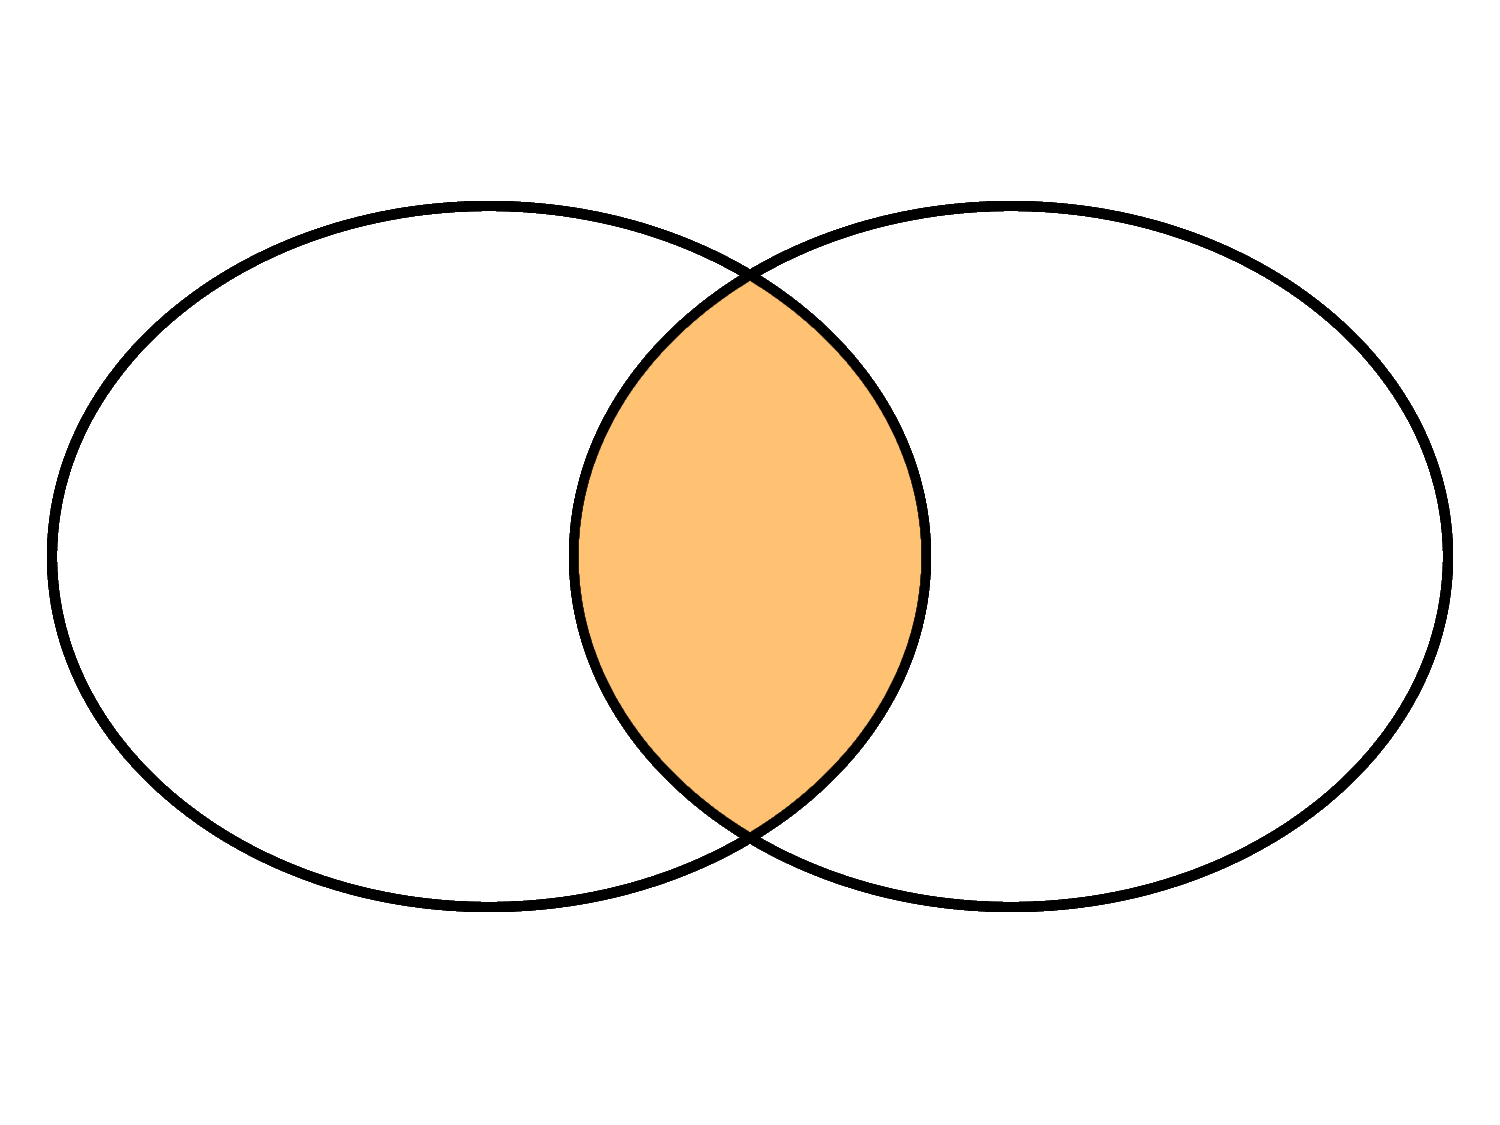
\includegraphics[width=0.7\textwidth]{figures/AundB.png}
    \caption{Veranschaulichung der Schnittmenge}
    \label{fig:my_label}
\end{figure}
\end{columns}
\end{frame}

\begin{frame}{Mengenoperationen - Vereinigung}
\begin{columns}
\column{0.5\textwidth}
    \begin{alertblock}{Vereinigung - $A\cup B$}
    Gegeben zwei Mengen A und B.\\
    In der Vereinigung liegt alles, das nur in A, nur in B \textbf{oder} in beiden Mengen liegt.
    \end{alertblock}
\column{0.5\textwidth}
\begin{figure}
    \centering
    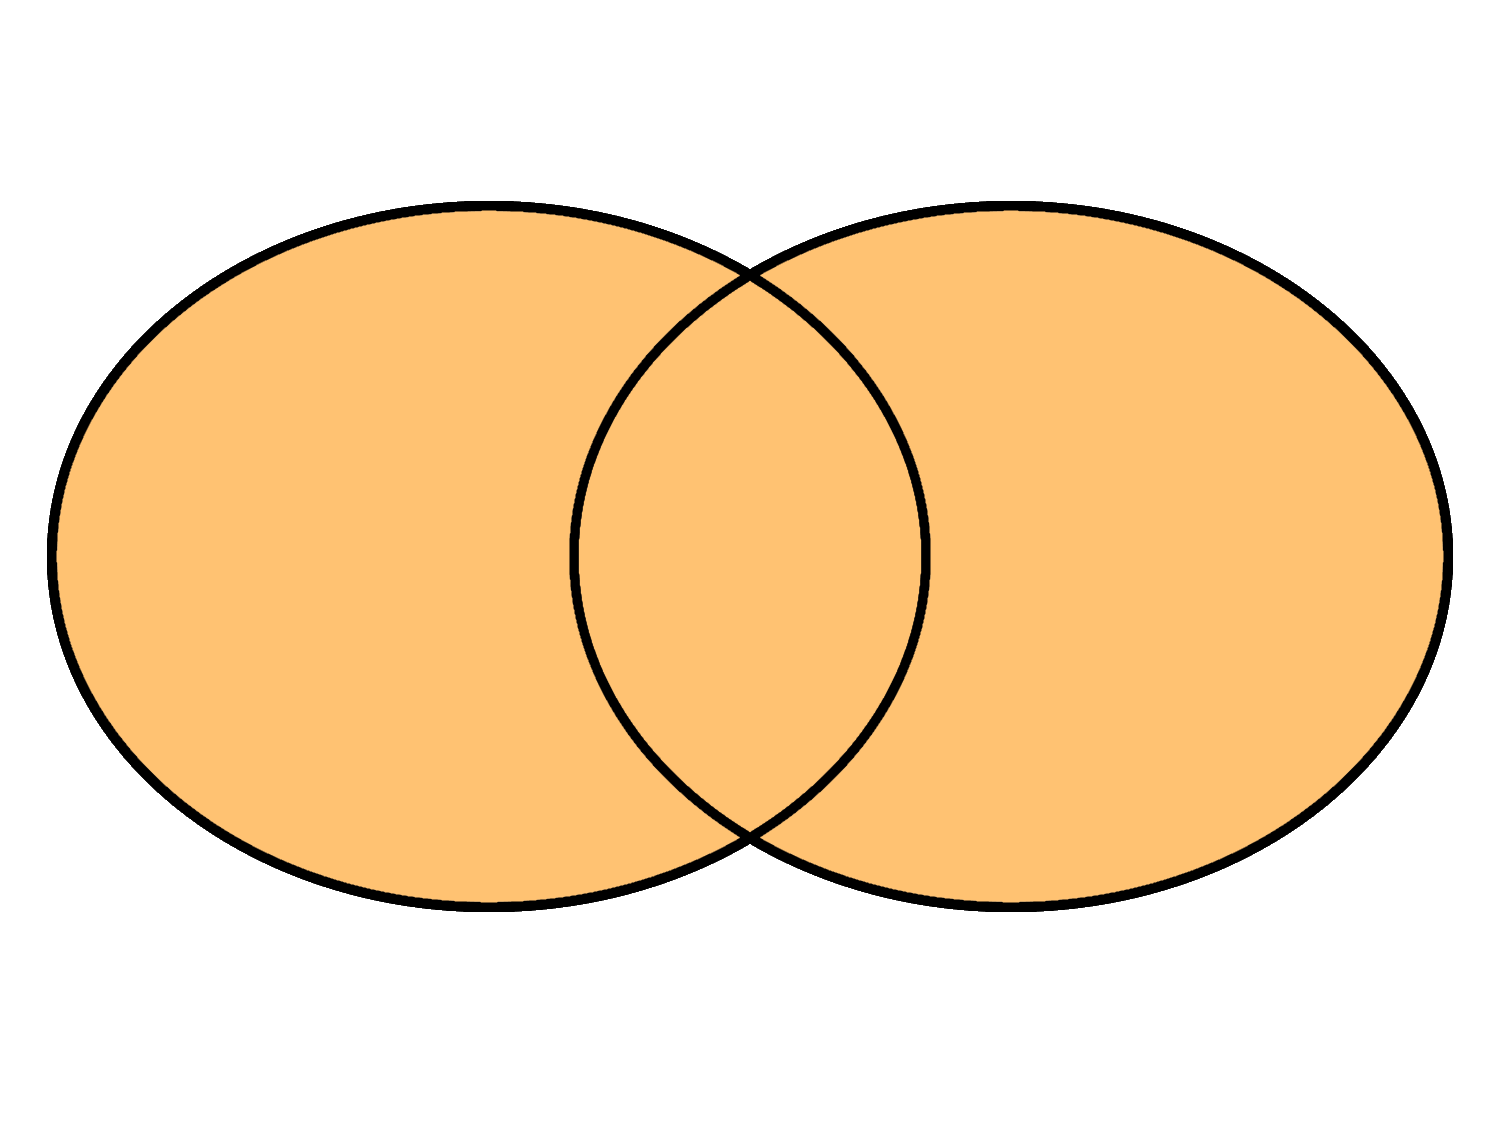
\includegraphics[width=0.7\textwidth]{figures/AoderB.png}
    \caption{Veranschaulichung der Vereinigung}
    \label{fig:my_label}
\end{figure}
\end{columns}
\end{frame}

\begin{frame}{Mengenoperationen - Komplement}
    \begin{columns}
\column{0.5\textwidth}
    \begin{alertblock}{Komplement - $\Bar{A}$}
    Gegeben sei eine Menge A.\\
    Im Komplement der Menge A liegen alle Elemente, die in $\Sigma^{*}$, aber nicht in der Menge A selbst liegen.
    \end{alertblock}
\column{0.5\textwidth}
\begin{figure}
    \centering
    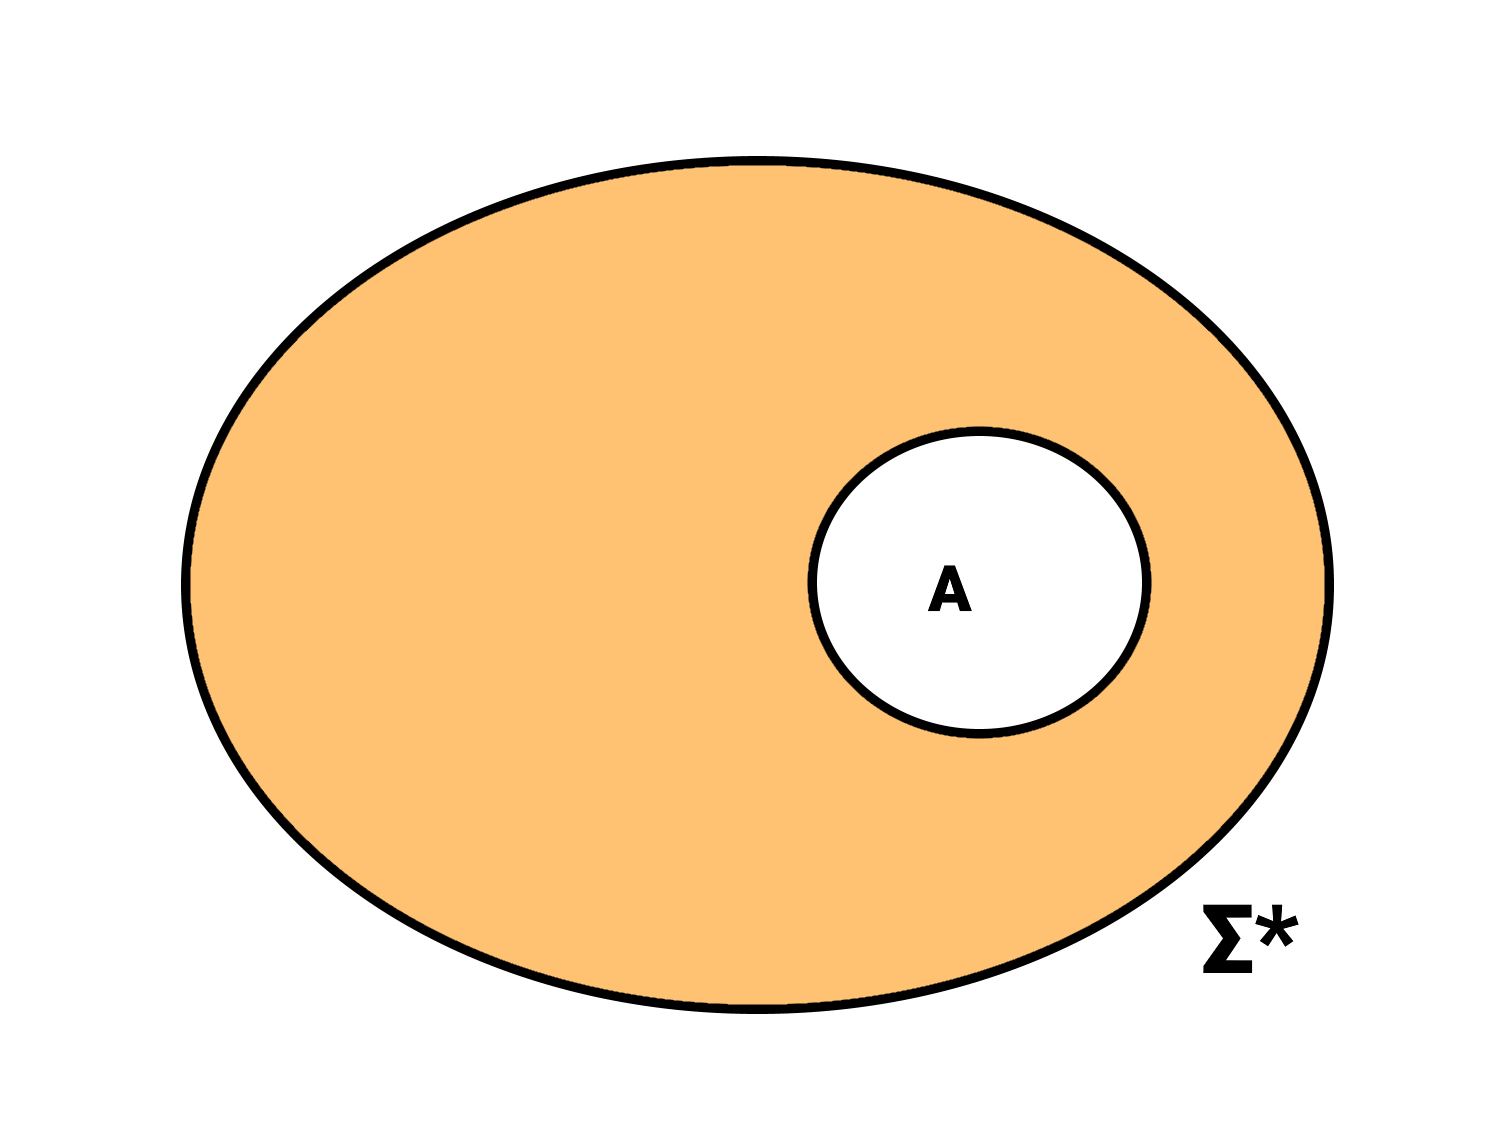
\includegraphics[width=0.7\textwidth]{figures/Akomp.png}
    \caption{Veranschaulichung des Komplements}
    \label{fig:my_label}
\end{figure}
\end{columns}
\onslide<2>{\alert{\emph{Anmerkung:}} Kann auch geschrieben werden als $\Sigma^{*}\setminus A$. \\
\hspace{2cm}(gesprochen $\Sigma^{*}$ \emph{\dq ohne"} $A$)}
\end{frame}

\begin{frame}{Mengenoperationen}
    Berechne folgende Mengen
    \metroset{block=fill}
    \begin{alertblock}{Normal}
        \begin{itemize}
            \item $M_1$: $\{a\}\cup \{b\}$
            \item $M_2$: $\{\} \cap \{u, v, w\}$
            \item $M_3$: $\mathbb{N} \cup \mathbb{Z}$
            \item $M_4$: $\overline{\{a^{n} | n \ \text{ist gerade}\} }$ , über dem Alphabet $\{a\}$
        \end{itemize}
    \end{alertblock}
        \begin{alertblock}{Schwer bis sehr schwer}
        \begin{itemize}
            \item $M_5$: $\{a, b, c\} \cap  \{a, \{b, c\}\}$
            \item $M_6$: $\{u \mid |u| \equiv 0 \mod 2, u \in \{a, b\}^{*}\}$\\\hspace{0.65cm}$\cup$ $\{v \mid |v| \equiv 0 \mod 4, v \in \{a, b\}^{*}\}$
            \item $M_7$: $\overline{\{a^{n} | n \ \text{ist gerade}\} }$ , über dem Alphabet $\{a,b\}$
        \end{itemize}
    \end{alertblock}
\end{frame}

{\setbeamercolor{palette primary}{bg=ExColor}
\begin{frame}{Lösungen}
  \begin{itemize}[<+- | alert@+>]
        \item 
            $M_1 = \{a, b\}$
        \item
            $M_2 = \emptyset$
        \item
            $M_3 = \mathbb{Z}$
        \item
            $M_4 = \{a^{n} \mid$ n ist ungerade$\}$, 
        \item
            $M_5 = \{a\}$
        \item
            $M_6 = \{u \mid |u| \equiv$ 0 mod 2$, u \in \{a, b\}^{*}\}$
        \item
            $M_7$: $\{a^{n} | n \ \text{ist ungerade}\} \cup\{w | w\in\{a,b\}, |w|_b>1\}$ 
    \end{itemize}
\end{frame}
}


\section{Wiederholung} 
\begin{frame}[fragile]{Das können wir jetzt beantworten}
    \begin{alertblock}{Einführung}
    \begin{itemize}
        \item Theoretische Informatik ist ganz schön wichtig...
        \item ...für mein Studium.
    \end{itemize}
    \end{alertblock}
\end{frame}

\begin{frame}[fragile]{Das können wir jetzt beantworten}
    \begin{alertblock}{Mengen, Sprachen, Elemente}
    \begin{itemize}
        \item Was ist eine Menge?
        \item Was ist eine Sprache?
        \item Was sind Elemente einer Sprache/Menge?
    \end{itemize}
    \end{alertblock}
\end{frame}

\begin{frame}[fragile]{Das können wir jetzt beantworten}
    \begin{alertblock}{Alphabete, $\SigmaStern$}
    \begin{itemize}
        \item Was ist ein Alphabet?, Was ist ein Wort?
        \item Wie funktioniert die Konkatenation?
        \item Was ist der Unterschied zwischen $\Sigma$ und $\SigmaStern$?
        \item Das leere Wort: Welches ist das \textit{kleinste} Alphabet, mit $\emptyWord \in \SigmaStern$?
        \item Bilden von $\SigmaStern$ für gegebenes Alphabet $\Sigma$
    \end{itemize}
    \end{alertblock}
\end{frame}

\begin{frame}[fragile]{Das können wir jetzt beantworten}
    \begin{alertblock}{Operationen auf Mengen}
    \begin{itemize}
        \item Wie funktionieren Vereinigung, Schnitt und Komplement?
        \item Wie bilde ich Vereinigungen oder Schnittmengen zweier Mengen?
        \item Wie bilde ich das Komplement einer Menge?
        \item Wie kann ich Sprachen formal beschreiben?
        \item Hantieren mit verschiedenen seltsamen Mengen und den Verknüpfungen
    \end{itemize}
    \end{alertblock}
\end{frame}

\begin{frame}[standout]
  Noch Fragen?
\end{frame}

\begin{frame}[fragile]{Glossar}
    \small
    \begin{tabular}{p{0.05\textwidth} p{0.25\textwidth} p{0.5\textwidth}}
    \toprule
    Abk.&Bedeutung&Was?!\\
    \midrule
        $\mathbb{N}$&natürliche Zahlen (mit 0)&In der theoretischen Informatik enthält $\mathbb{N}$ die 0: $\mathbb{N}=\{0,1,2,3,\dots\}$\\
        $\mathbb{Z}$&ganze Zahlen&\\
        $\mathbb{Q}$&rationale Zahlen&können als Bruch dargestellt werden\\
        $\Sigma$ & Sigma& mit diesem Zeichen wird oft das Alphabet (die Menge an verwendbaren Symbolen) repräsentiert\\
        $\Sigma^\ast$&Sigma Stern&Menge aller Möglichkeiten Elemente aus $\Sigma$ hintereinander zu schreiben\\
        $\emptyset$&\{\}&leere Menge\\
        :&sodass&z.B. $\forall a,b\in\mathbb{Z}:$a teilt b\\
    \bottomrule
    \end{tabular}
\end{frame}

\end{document}